\let\negmedspace\undefined
\let\negthickspace\undefined
\documentclass[journal]{IEEEtran}
\usepackage[a5paper, margin=10mm, onecolumn]{geometry}
%\usepackage{lmodern} % Ensure lmodern is loaded for pdflatex
\usepackage{tfrupee} % Include tfrupee package

\setlength{\headheight}{1cm} % Set the height of the header box
\setlength{\headsep}{0mm}     % Set the distance between the header box and the top of the text

\usepackage{gvv-book}
\usepackage{gvv}
\usepackage{cite}
\usepackage{amsmath,amssymb,amsfonts,amsthm}
\usepackage{algorithmic}
\usepackage{graphicx}
\usepackage{textcomp}
\usepackage{xcolor}
\usepackage{txfonts}
\usepackage{listings}
\usepackage{enumitem}
\usepackage{mathtools}
\usepackage{gensymb}
\usepackage[breaklinks=true]{hyperref}
\usepackage{tkz-euclide} 
\usepackage{listings}
% \usepackage{gvv}                                        
\def\inputGnumericTable{}                                 
\usepackage[latin1]{inputenc}                                
\usepackage{color}                                            
\usepackage{array}                                            
\usepackage{longtable}                                       
\usepackage{calc}                                             
\usepackage{multirow}                                         
\usepackage{hhline}                                           
\usepackage{ifthen}                                           
\usepackage{lscape}
\usepackage{circuitikz}
\usepackage{comment}
\tikzstyle{block} = [rectangle, draw, fill=blue!20, 
    text width=4em, text centered, rounded corners, minimum height=3em]
\tikzstyle{sum} = [draw, fill=blue!10, circle, minimum size=1cm, node distance=1.5cm]
\tikzstyle{input} = [coordinate]
\tikzstyle{output} = [coordinate]


\begin{document}

\bibliographystyle{IEEEtran}
\vspace{3cm}

\title{10.7.75}
\author{EE25BTECH11026-Harsha}
 \maketitle
% \newpage
% \bigskip
{\let\newpage\relax\maketitle}

\renewcommand{\thefigure}{\theenumi}
\renewcommand{\thetable}{\theenumi}
\setlength{\intextsep}{10pt} % Space between text and floats


\numberwithin{equation}{enumi}
\numberwithin{figure}{enumi}
\renewcommand{\thetable}{\theenumi}

\textbf{Question}:\\
Find the equations of tangents drawn from origin to the circle $x^2+y^2-2rx-2hy+h^2=0$,are
\begin{multicols}{2}
\begin{enumerate}
    \item $x=0$
    \item $y=0$
    \item $\brak{h^2-r^2}x-2rhy=0$
    \item $\brak{h^2-r^2}x+2rhy=0$
\end{enumerate}
\end{multicols}
\solution \\
Let us solve the given question theoretically and then verify the solution computationally.\\
\\
Given the equation of circle,
\begin{align}
    \vec{x}^{\top}\vec{V}\vec{x}+2\vec{u}^{\top}\vec{x}+f=0 \label{eq:1}
\end{align}
where, $\vec{x}=\myvec{x\\y}$,$\vec{V}=\myvec{1&&0\\0&&1}$,$\vec{u}=\myvec{-r\\-h}$ and $f=h^2$.\\ 
\\
It is given that the tangents pass through the origin.
\begin{align}
    \therefore \vec{n}^{\top}\vec{x}=0 \label{eq:2}
\end{align}
where $\vec{n}$ is the direction vector of the tangent.\\
\\
It is known that for any conic , the condition of tangency is given by,
\begin{align}
    \vec{n}^{\top}\vec{\Sigma}\vec{n}=0 \label{eq:3}
\end{align}
where,
\begin{align}
    \vec{n}=\myvec{1\\m}\brak{\text{Direction vector of tangent}}
\end{align}
\begin{align}
   \vec{\Sigma}=\brak{\vec{V}\vec{h}+\vec{u}}\brak{\vec{V}\vec{h}+\vec{u}}^{\top}-S\brak{\vec{h}}\vec{V} \label{eq:4}
\end{align}
$\vec{h}$ is the point through which the tangent passes and $S\brak{\vec{h}}=\vec{h}^{\top}\vec{V}\vec{h}+2\vec{u}^{\top}\vec{h}+f=0$.\\
From ~\eqref{eq:2}, ~\eqref{eq:4} reduces to,
\begin{align}
    \vec{\Sigma}=\vec{u}\vec{u}^{\top}-f\vec{V}
\end{align}
yielding,
\begin{align}
    \vec{n}^{\top}\brak{\vec{u}\vec{u}^{\top}-f\vec{V}}\vec{n}=0
\end{align}
\newpage
\vspace*{0.25cm}
\begin{align}
    \implies \vec{n}^{\top}\vec{u}\vec{u}^{\top}\vec{n}-f\vec{n}^{\top}\vec{V}\vec{n}=0 
\end{align}
\begin{align}
    \therefore \|\vec{u}^{\top}\vec{n}\|^2=f\vec{n}^{\top}\vec{V}\vec{n} \label{eq:5}
\end{align}
Substituting $\vec{V}$ in ~\eqref{eq:5},
\begin{align}
    \implies \|\vec{u}^{\top}\vec{n}\|^2=f\|\vec{n}\|^2
\end{align}
\begin{align}
    \implies \brak{rm+h}^2=h^2\brak{1+m^2}
\end{align}
\begin{align}
    \therefore m\brak{\brak{r^2-h^2}m-2rh}=0
\end{align}
\begin{align}
    \implies \vec{n}=\myvec{1\\0} \qquad \vec{n}=\myvec{h^2-r^2\\-2rh}
\end{align}
\\
From the figure, it is clearly verified that the theoretical solution matches with the computational solution.\\

\begin{figure}[H]
    \centering
    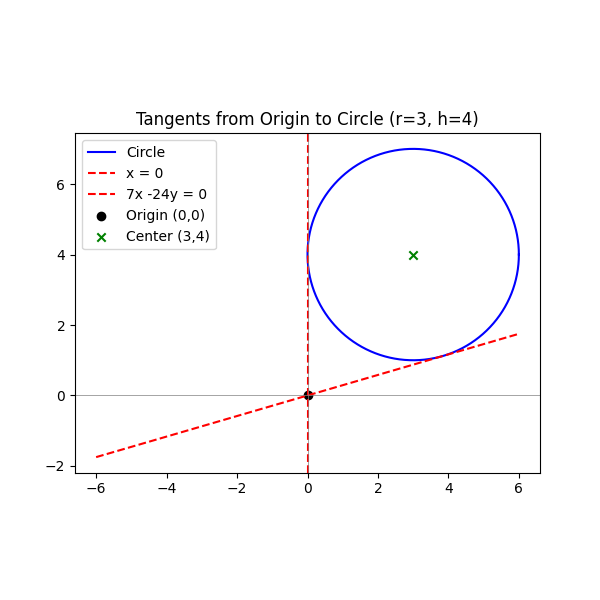
\includegraphics[width=0.6\columnwidth]{figs/Figure_1.png}
    \label{fig:1}
\end{figure}

\end{document}
